
\section{Merging Beyond Identical Functions}

In the previous sections, we have seen compiler optimisations that merge identical functions.
However, nearly identical functions, with only minor differences, are also commonly found.
Figure~\ref{fig:example-similar} shows two examples of nearly identical functions found in real programs.
The highlighted differences prevent these functions from being merged by the identical function merging techniques.
%These functions are usually produced by copy-and-paste programming,
%where a given code pattern is copied and then repurposed~\cite{kim04,jablonski10,ahmed15}.
The first pair of functions, shown in Figure~\ref{fig:example-similar-1-hmmer}, illustrates code that is usually produced by copy-and-paste programming,
where a given code pattern is copied and then repurposed~\cite{kim04,jablonski10,ahmed15}.
The second pair of functions, shown in Figure~\ref{fig:example-similar-3-gcc}, are produced by generative programming~\cite{czarnecki99,draheim04}, where their code was
automatically generated using a description language~\cite{ghica15}.

\begin{figure}[h]
\centering
\begin{subfigure}{\textwidth}
\centering
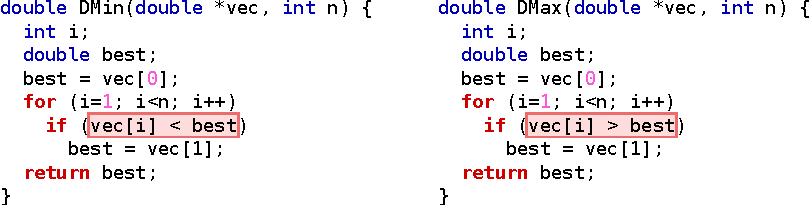
\includegraphics[width=0.9\textwidth]{src/relatedwork/figs/example-similar-1-hmmer}
\caption{Two similar functions extracted from the \texttt{456.hmmer} benchmark.}
\label{fig:example-similar-1-hmmer}
\end{subfigure}
%\begin{subfigure}{\textwidth}
%\centering
%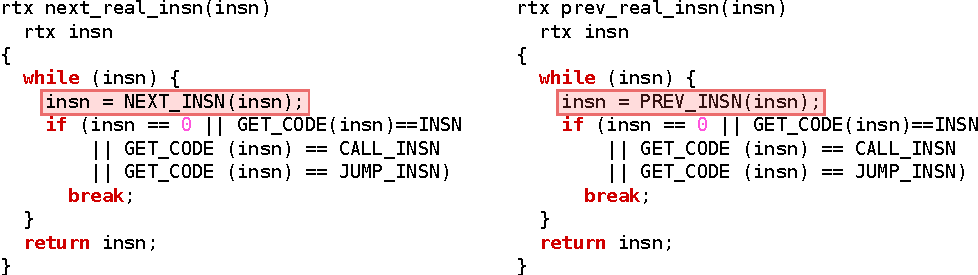
\includegraphics[width=0.9\textwidth]{src/relatedwork/figs/example-similar-2-gcc}
%\caption{Two similar functions extracted from the \texttt{403.gcc} benchmark.}
%\label{fig:example-similar-2-gcc}
%\end{subfigure}
\begin{subfigure}{\textwidth}
\centering
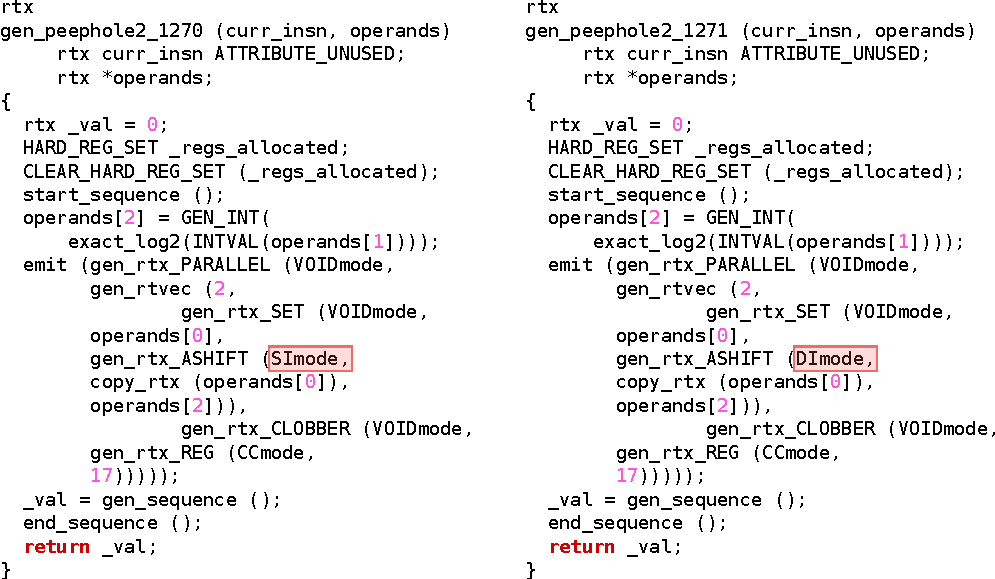
\includegraphics[width=\textwidth]{src/relatedwork/figs/example-similar-3-gcc}
\caption{Two similar functions extracted from the \texttt{403.gcc} benchmark.}
\label{fig:example-similar-3-gcc}
\end{subfigure}
\caption{Example of two pairs of highly similar functions. Because they are not identical, they cannot be merged by the function merging technique currently found in major compilers.}
\label{fig:example-similar}
\end{figure}


% The function merging technique presented in \cite{edler14} restricts merging to nearly identical functions.
% They only allow for pairs of corresponding instructions to differ if they still have equivalent data type.


Von Edler~et~al.~\cite{edler14} have proposed a function-merging technique exploits structural similarity among functions.
Their optimization is able to merge nearly identical functions.
%similar functions that are not necessarily identical.
Two functions are structurally similar if both their function types are equivalent
and their CFGs isomorphic.
Two function types are equivalent if they agree in the number, order, and types
of their parameters as well as
their return types, linkage type, and other compiler-specific properties.
In addition to the structural similarity of the functions, their technique also
requires that corresponding basic blocks have exactly the same number of instructions
and that corresponding instructions must have equivalent resulting types.
% but may differ in their opcodes or in the number and type of their input operands.
Mergeable functions are only allowed to differ in corresponding instructions,
where they can differ in their opcodes or in the number and type of their input operands.
Corresponding named values must have the same data type.
%The only differences that are actually allowed is that
%corresponding instructions can 
%differ in their opcodes or in the number and type of their input operands.


%If two corresponding instructions have different opcodes, they split the basic
%block and insert a switch branch to select which instruction to execute
%depending on a function identifier.

Because the state-of-the-art is limited to functions with identical CFGs
and function types, once it merges a pair of functions, a third
\textit{similar} function cannot be merged into the resulting merged function
since they will differ in both CFGs and their lists of parameters.
Due to this limiting factor, the state-of-the-art has to first group
mergeable functions before simultaneously merging all functions within a group.

The state-of-the-art algorithm iterates simultaneously over corresponding basic
blocks in the set functions being merged, as they have isomorphic CFGs.
Figure~\ref{fig:soa-example-1} shows an example of two functions with isomorphic CFGs and their corresponding basic blocks arranged side by side.

\begin{figure}[h]
  \centering
  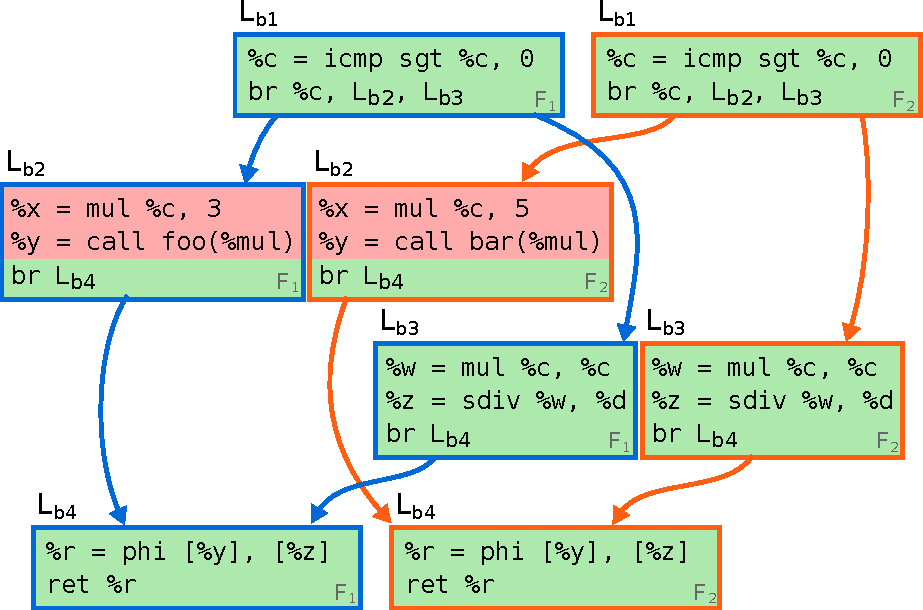
\includegraphics[width=0.8\textwidth]{src/relatedwork/figs/soa-example-1.pdf}
  \caption{An example of two functions with isomorphic CFGs and their corresponding basic blocks arranged side by side. Instructions in paired basic blocks are compared in a pairwise manner.}
  \label{fig:soa-example-1}
\end{figure}

Every pair of basic blocks have their instructions analysed in a pairwise manner.
Two instructions match if they have the same opcode with equivalent data types and operands.
Even if two instructions differ only on their operands, they are classified as mismatching.
For every pair of basic blocks, if their corresponding instructions have any difference, except for the data type of the computed value, the merged basic block is split by inserting a switch branch to select which instruction
to execute depending on a function identifier.
A phi-node is used to unify the mismatching instructions as a single named value.
This unification is only possible because they compute values of the equivalent data types.
Note that no operand selection is performed, every use of the mismatching instructions will refer to their phi-node.
Figure~\ref{fig:soa-example-2} shows an example of a merged basic block containing two mismatching pairs of instructions.
A split is added for every pair of mismatching instructions with the phi-node instruction added to the their immediate point of convergence.

% Because these instructions have equivalent resulting types, their results can be
% merged using a phi-operator, which can then be used transparently as operands
% by other instructions.

\begin{figure}[h]
  \centering
  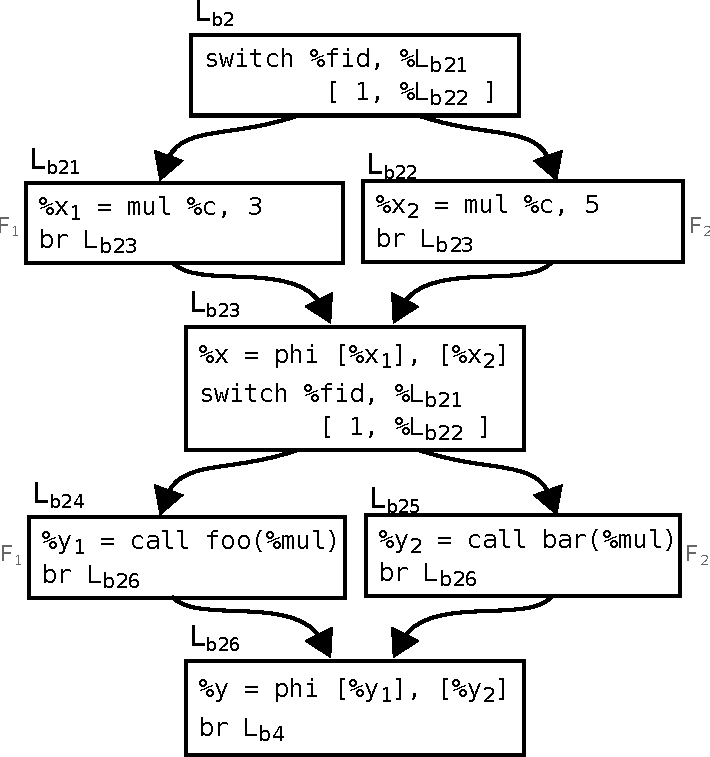
\includegraphics[width=0.6\textwidth]{src/relatedwork/figs/soa-example-2.pdf}
  \caption{An example of a merged basic block containing two mismatching pairs of instructions. A split is added for every pair of mismatching instructions with the phi-node instruction added to the their immediate point of convergence.}
  \label{fig:soa-example-2}
\end{figure}

Overall, except for mismatching pairs of instructions, the two functions must have identical function types, i.e., they must have the same return type and list of arguments, identical CFGs, with corresponding basic blocks having the same number of instructions.
Although this technique improves over LLVM's identical function merging, it is
still unnecessarily limited.
In Section~\ref{sec:motivation}, we showed examples of very similar real functions where the state-of-the-art fails to merge.
In Chapter~\ref{chp:cgo19} we introduce a novel technique that addresses such limitations improving on the state-of-the-art across the board.

%%%%%%%%%%%%%%%%%%%%%%%%%%%%%%%%%%%%%%%%%%%%%%%%%%%%%%%%%%%%%%%%%%%%%%%%

